\begin{sidewaystable}
%\begin{table}[htdp]
\caption{Resolving the top hat function in two different polynomial bases.}
\begin{center}
\begin{tabular}{cccc}
 %
   order & fit vs. ideal & Zernike amplitudes $\alpha_{2k}$ & monomial amplitudes $a_{2k}$ \\[10pt]
 %
   $10$ &
   \raisebox{-0.5\height}{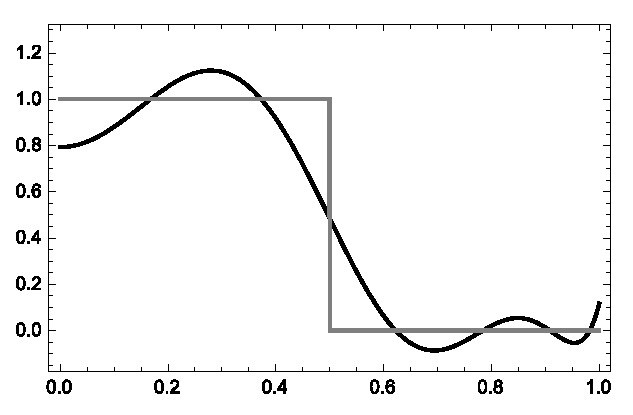
\includegraphics[ width = 2.25in ]{graphics/fit_010.eps}} &
   \raisebox{-0.5\height}{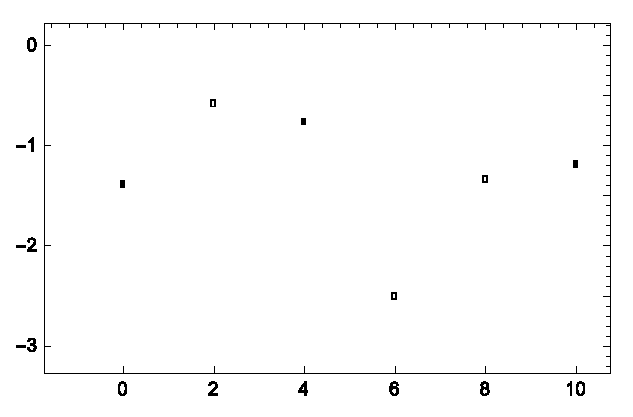
\includegraphics[ width = 2.25in ]{graphics/amps_Zernike_010.eps}} &
   \raisebox{-0.5\height}{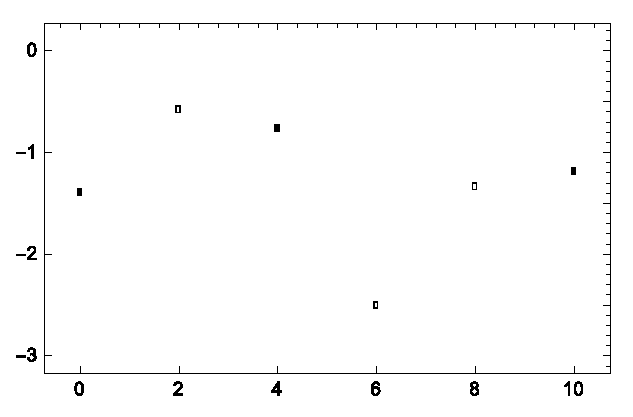
\includegraphics[ width = 2.25in ]{graphics/amps_monomial_010.eps}} \\[15pt]
 %
   $100$ &
   \raisebox{-0.5\height}{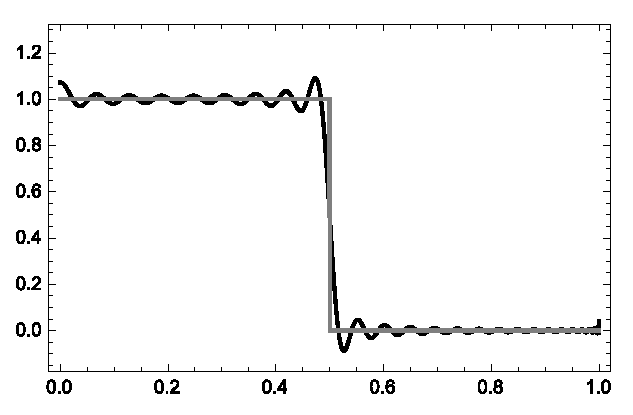
\includegraphics[ width = 2.25in ]{graphics/fit_100.eps}} &
   \raisebox{-0.5\height}{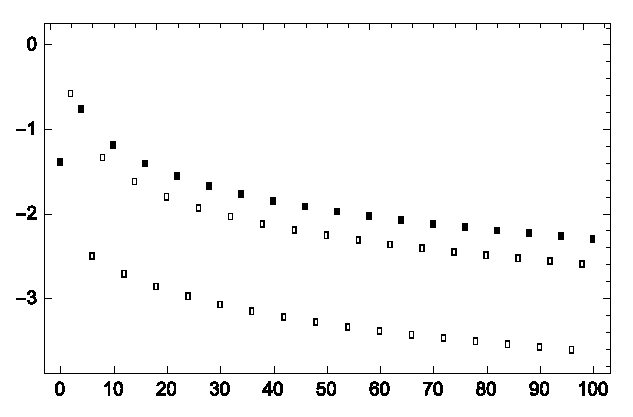
\includegraphics[ width = 2.25in ]{graphics/amps_Zernike_100.eps}} &
   \raisebox{-0.5\height}{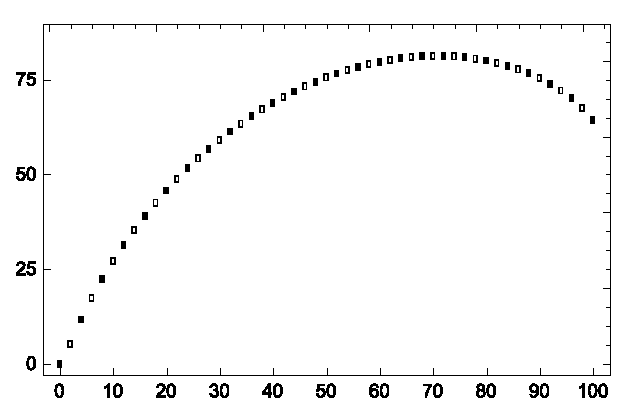
\includegraphics[ width = 2.25in ]{graphics/amps_monomial_100.eps}} \\[15pt]
 %
   $200$ &
   \raisebox{-0.5\height}{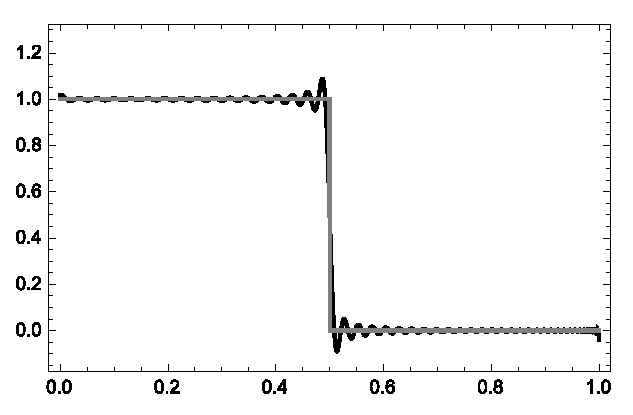
\includegraphics[ width = 2.25in ]{graphics/fit_200.eps}} &
   \raisebox{-0.5\height}{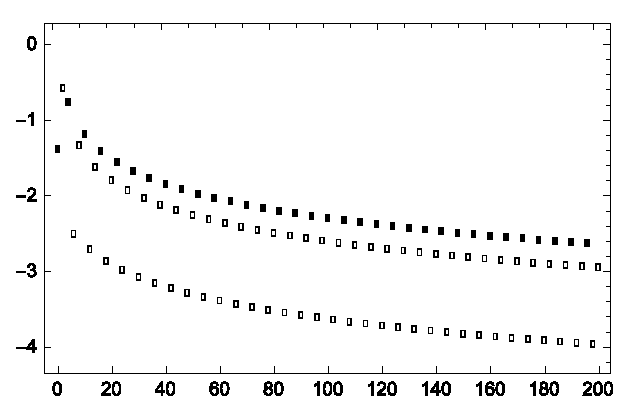
\includegraphics[ width = 2.25in ]{graphics/amps_Zernike_200.eps}} &
   \raisebox{-0.5\height}{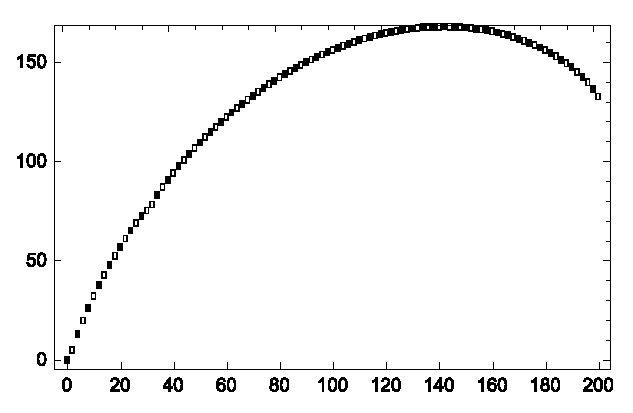
\includegraphics[ width = 2.25in ]{graphics/amps_monomial_200.eps}} \\
 %
 %
 %
\end{tabular}
\end{center}
\label{tab:top hat fit}
%\end{table}

\end{sidewaystable}

\endinput %-------------------------------